\chapter{Les normes et le raisonnement juridique}
\section{Hiérarchie des normes}
\subsection{Définition}
\large{
\textbf{Le droit} est un ensemble de \textbf{règles} qui organisent la vie en société et régissent \textbf{les relations entre les individus, les institutions et l'état.}
Ces règles sont créées par des \textbf{autorités compétentes}, comme le législateur, et sont appliquées par des tribunaux ou d'autres institutions de justice \newline

Le droit est divisé en plusieurs branches, comme : \newline

}
\begin{itemize}
    \item \textbf{Le droit civil} : concerne les relations entre les particuliers, par exemple en matière de mariage, de propriétés ou de contrats
    \item \textbf{Le droit pénal} : détermine les infractions (crimes, délits, contraventions) et fixe les sanctions applicables
    \item \textbf{Le droit administratif} : encadre les relations entre les citoyens et les administrations publiques
    \item \textbf{Le droit internationnal} : régit les relations entre les états et questions juridiques dépassant les frontières nationnales
    \item \textbf{Le droit commercial} : concerne les activités économiques, les entreprises et les transactions commerciales
\end{itemize}
En cas de non respect de ces règles, le citoyen encours des sanctions. Le droit peut évoluer dans le temps en fonction des changements sociaux, technologiques ou économiques
\begin{center}
    \begin{figure}[hbt!]
        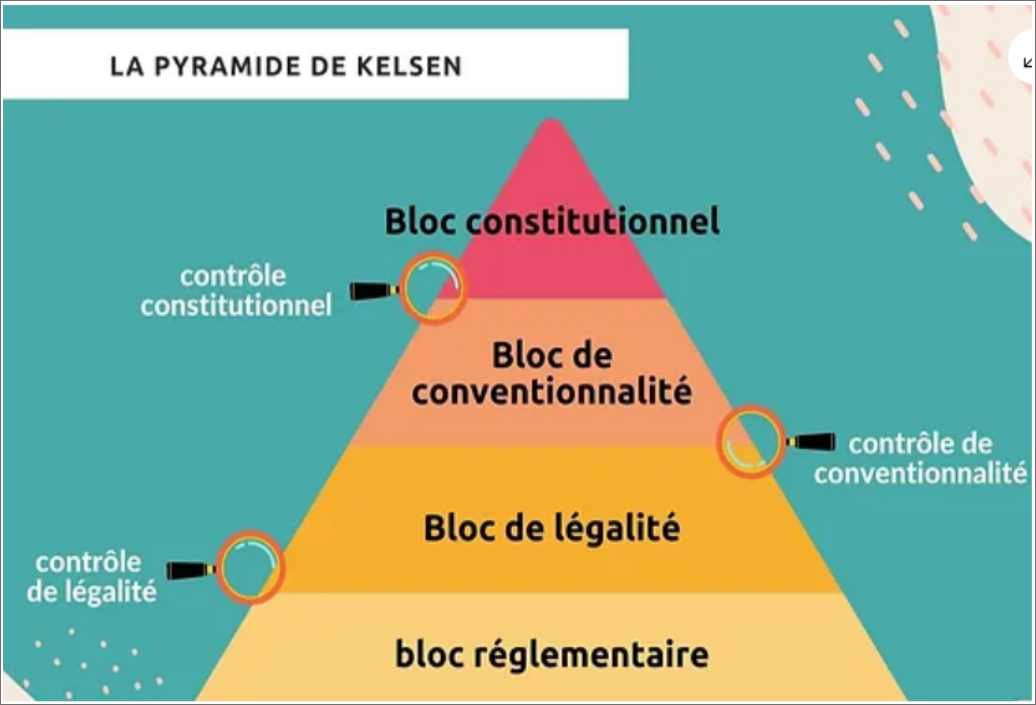
\includegraphics[scale=0.4]{Pics/Pyramide_de_Kelsen.png}
        \caption{Hiérarchie des normes}
    \end{figure}
\end{center}
\newpage
\section{Les normes}
Les \textbf{normes juridiques} sont à différentier des \textbf{normes sociales}. Une norme juridique est une règle qui établit une source de droits et d'obligations juridiques tandis
qu'une norme sociale provient d'une tradition, de la morale lorsqu'un individu se socialise. 
\subsection{Bloc constitutionnel}
C'est la Constitution : un ensemble de normes juridiques, de principes et de règles appliquées par le conseil constitutionnel. \footnote{Vérifie la conformité des lois à la Constitution}
\begin{center}
    \begin{figure}[hbt!]
        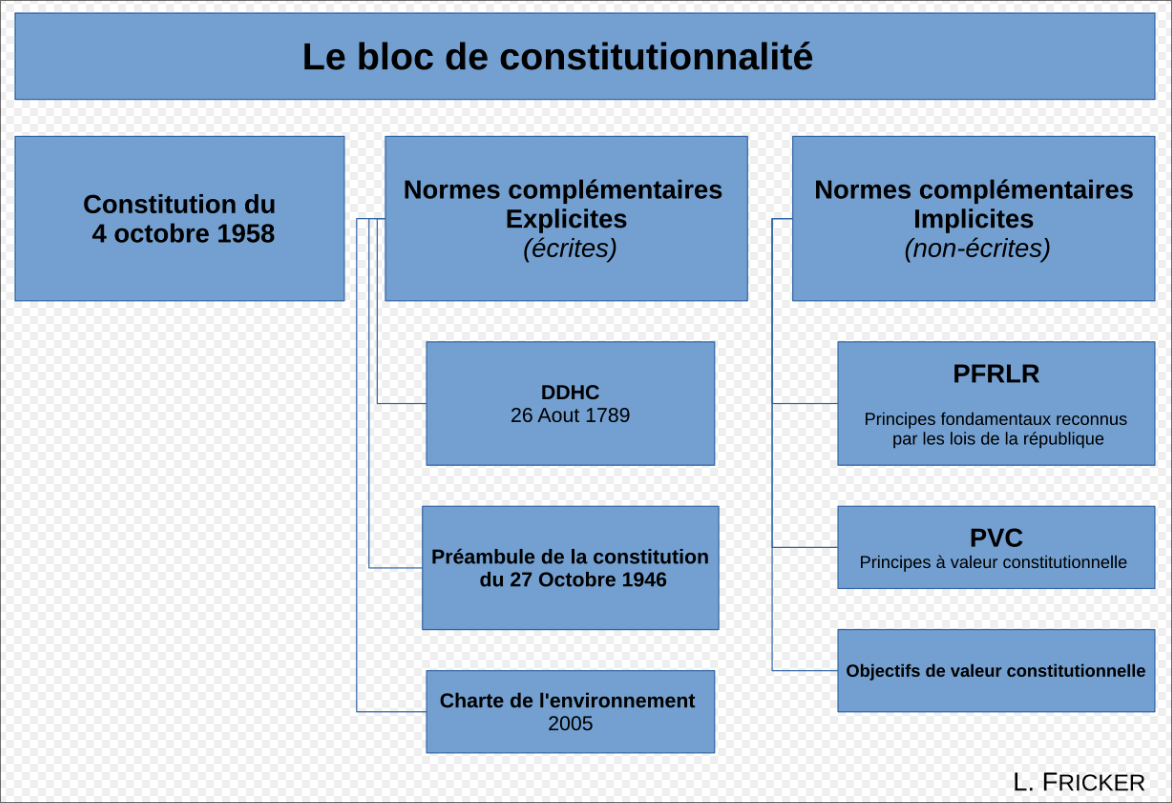
\includegraphics[scale=0.3]{Pics/Bloc_de_constitutionnalite.png}
        \caption{Bloc constitutionnel}
    \end{figure}
\end{center}
\newpage
\subsection{Bloc conventionnel}
\textbf{Le bloc de conventionnalité l'ensemble des traités et conventions entre les Etats ou entre mes Etats et les organisations internationnales} \newline
Exemple : l'\textbf{UE} est une organisation économique et politique qui rasssemble 27 états membres. Elle a pour but de promouvoir la paix, la stabilité et la coopération économique entre les états memebres. \newline
\begin{center}
    \begin{figure}[hbt!]
        
\includegraphics[scale=0.3]{Pics/Institutions_UE.png}
        \caption{Illustration des institutions dans l'Union Européenne}
    \end{figure}
\end{center}
\newpage
